\section{Laplace: Analysis Becomes the Language of the Universe (1799)}

If Euler revealed that motion and oscillation could be written in the elegant script of exponentials, then \textbf{Pierre-Simon Laplace} took that script and declared it sufficient to describe \textit{everything}.

Where Euler transformed trigonometry, Laplace transformed \textbf{mathematical analysis} itself—elevating it from a tool for solving problems to a universal framework for predicting the future.

\subsection{From Euler and Lagrange to Laplace}

Euler’s analytic legacy didn’t end with exponentials. Alongside \textbf{Joseph-Louis Lagrange}, he laid the foundation for a new kind of mechanics—one that replaced Newton’s geometric forces with equations of motion derived from principles of least action.

At the heart of this was the \textbf{Euler-Lagrange equation}, a powerful statement that the behavior of physical systems could be deduced by optimizing a functional:

\[
\frac{d}{dt} \left( \frac{\partial L}{\partial \dot{q}} \right) - \frac{\partial L}{\partial q} = 0
\]

But while Euler and Lagrange provided the machinery, it was Laplace who fully embraced its philosophical consequences.

\subsection{Laplace’s Deterministic Vision}

Laplace extended this analytic framework beyond isolated systems. To him, the success of mathematics in celestial mechanics was no accident—it was a revelation. The same equations that governed planetary orbits could, in principle, govern \textit{all phenomena}, from falling apples to human thought.

In 1799, Laplace famously articulated his vision:

\begin{quote}
\textit{“We ought to regard the present state of the universe as the effect of its past and the cause of its future...  
An intellect which at a certain moment knew all forces and positions...  
nothing would be uncertain, and the future, as the past, would be present to its eyes.”}
\end{quote}

This was more than philosophy—it was a declaration that **mathematical analysis had become the language of nature itself**.

\subsection{The Laplacian Expansion of Analysis}

Laplace didn’t just theorize determinism—he built the analytic tools to support it:

\begin{itemize}
    \item He extended the use of **differential equations** to describe gravitational systems with exquisite precision.
    \item He developed what we now call the **Laplace Transform**, turning complex dynamical problems into algebraic ones—a method that would later become essential in engineering and physics.
    \item He formalized **probability theory** as a branch of analysis, framing uncertainty not as a flaw in knowledge, but as a calculable measure of ignorance.
\end{itemize}

\begin{figure}[H]
    \centering
    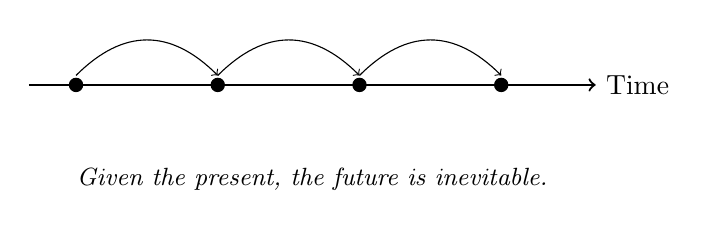
\begin{tikzpicture}[scale=1.2]
      % Representing deterministic flow
      \draw[->, thick] (0,0) -- (6,0) node[right] {Time};
      
      % States along timeline
      \foreach \x in {0.5, 2, 3.5, 5} {
        \filldraw (\x,0) circle (2pt);
      }
      
      % Arrows showing causality
      \foreach \x in {0.5, 2, 3.5} {
        \draw[->] (\x,0.1) .. controls +(0.5,0.5) and +(-0.5,0.5) .. (\x+1.5,0.1);
      }
      
      \node at (3,-1) {\small \textit{Given the present, the future is inevitable.}};
    \end{tikzpicture}
    \caption{Laplace’s Determinism: Every state of the universe flows from precise mathematical relations.}
\end{figure}

\subsection{From Curves to Causes}

Barrow saw geometry. Euler saw formulas. But Laplace saw something far more ambitious:

\begin{center}
\textit{The universe itself as an analytic expression—  
a seamless web of differential equations waiting to be solved.}
\end{center}

For Laplace, mathematical analysis was no longer just a method for solving isolated problems—it was a **theory of everything**, centuries before that phrase was coined.

\vspace{1em}

His work marks the moment when analysis stopped being a servant of physics and became its master—capable, in theory, of predicting the dance of galaxies or the fall of a leaf with equal precision.

Of course, Laplace’s demon—the hypothetical intellect that could compute the future—never materialized. But his legacy did:  
Every time we write down a differential equation, optimize a system, or transform a problem into solvable terms, we’re speaking the language that Laplace helped define.

